%!TEX program = lualatex
\documentclass[12pt, a4paper]{report}

% --- Packages ---
\usepackage{fontspec}
\setmainfont{Times New Roman}
\usepackage{amsmath, amssymb, amsfonts, mathtools}
\usepackage{geometry}
\geometry{top=2.5cm, bottom=2.5cm, left=3cm, right=2cm}
\usepackage{setspace}
\usepackage{booktabs}
\usepackage{multirow}
\usepackage{multicol}
\usepackage{tabularx}
\usepackage{tikz}
\usepackage{pgfplots}
\pgfplotsset{compat=1.18}
\usepackage{titlesec}
\usepackage{tocloft}
\usepackage{enumitem}
\usepackage{xcolor}
\usepackage{listings}
\usepackage{algorithm}
\usepackage{algorithmic}
\usepackage{indentfirst}
\usepackage{graphicx}
\usepackage{subcaption}
\usepackage[colorlinks=true, linkcolor=blue, urlcolor=blue, citecolor=blue]{hyperref}

% Captions & tables
\usepackage{longtable}
\usepackage{caption}
\usepackage{url}
\usepackage{cleveref}
\usepackage{tcolorbox}
\usepackage{lmodern}
\usepackage{array}

\newcommand{\HRule}{\rule{\linewidth}{1pt}}

\begin{document}

% --- Thay đổi margin tạm thời để trang bìa nằm ở giữa giấy ---
\newgeometry{top=2.5cm, bottom=2.5cm, left=2.5cm, right=2.5cm}

% --- TITLE PAGE ---
\begin{titlepage}
    \centering
    \vspace*{0.5cm}
    {\large \textbf{ĐẠI HỌC QUỐC GIA THÀNH PHỐ HỒ CHÍ MINH}}\\[0.5cm]
    {\large \textbf{TRƯỜNG ĐẠI HỌC CÔNG NGHỆ THÔNG TIN}}\\[1.5cm]

    % Logo trường
    
\includegraphics[scale=0.7]{images/logo-uit.png}\\[1.5cm]

    {\Large \textbf{KHOA HỆ THỐNG THÔNG TIN}}\\[0.5cm]
    {\large \textbf{IS353 - PHÂN TÍCH MẠNG XÃ HỘI}}\\[1cm]

    \HRule \\[0.4cm]
    \makebox[\textwidth][c]{\textbf{\large ĐỒ ÁN:}}\\[0.3cm]
    \textbf{\Large DEVICE-CLOUD COLLABORATIVE LEARNING
    FOR GRAPH NEURAL NETWORKS IN\\[0.2cm]
    PERSONALIZED RECOMMENDATION SYSTEMS}\\[0.2cm]
    \HRule \\[1.5cm]

    % --- STUDENT AND INSTRUCTOR SIDE-BY-SIDE LAYOUT ---
    \vspace{0.5cm}
    \noindent
    \begin{minipage}[t]{0.62\textwidth}
        \large
        \textbf{Nhóm sinh viên thực hiện:}\\[0.2cm]
        \normalsize
        1. Nguyễn Quang Dũng - 23520335 (Nhóm trưởng)\\[0.1cm]
        2. Trần Nguyễn Tiến Đức - 23520322\\[0.1cm]
        3. Lê Bá Vinh - 22521670\\[0.1cm]
        4. Huỳnh Khánh Bảo - 23520101
    \end{minipage}%
    \begin{minipage}[t]{0.38\textwidth}
        \large
        \centering
        \textbf{Giảng viên hướng dẫn:}\\[0.2cm]
        \normalsize
        % TODO: Điền tên giảng viên
        ThS. Hà Lê Hoài Trung
    \end{minipage}

    \vfill
    {\large TP. Hồ Chí Minh, 2026}
\end{titlepage}

% --- Khôi phục lại margin ban đầu (trái 3cm) để đóng gáy ---
\restoregeometry

\newpage
\pagenumbering{roman}
\renewcommand{\contentsname}{Mục lục}
\tableofcontents
\newpage
\pagenumbering{arabic}

% -- CHƯƠNG 1: Giới thiệu
\chapter{GIỚI THIỆU}

\section{Lý do chọn đề tài}

Trong kỷ nguyên số hiện nay, sự bùng nổ của các nền tảng thương mại điện tử và mạng xã hội đã dẫn đến sự quá tải thông tin đối với người tiêu dùng. Hệ thống khuyến nghị (Recommender Systems - RS) đã trở thành một thành phần không thể thiếu, đóng vai trò quan trọng trong việc cá nhân hóa trải nghiệm và hỗ trợ người dùng tìm kiếm sản phẩm, dịch vụ phù hợp giữa hàng triệu lựa chọn. Tuy nhiên, các hệ thống khuyến nghị truyền thống dựa trên kiến trúc tập trung (Cloud-Centric) đang đối mặt với ba thách thức lớn:

\begin{itemize}
    \item \textbf{Rủi ro về quyền riêng tư (Privacy Risks):} Việc tải toàn bộ nhật ký hành vi thô của người dùng (như click, view, mua sắm) lên máy chủ đám mây tiềm ẩn nguy cơ rò rỉ thông tin cá nhân nhạy cảm, gây lo ngại lớn trong bối cảnh các quy định về bảo vệ dữ liệu (như GDPR) ngày càng thắt chặt.
    \item \textbf{Độ trễ và khả năng thích ứng thời gian thực (Latency \& Real-time Adaptivity):} Các mô hình tập trung thường gặp khó khăn trong việc cập nhật tức thời sự thay đổi trong sở thích người dùng do độ trễ truyền tải dữ liệu và thời gian xử lý tại server, làm giảm hiệu quả của các khuyến nghị mang tính ngữ cảnh.
    \item \textbf{Chi phí truyền tải và tài nguyên (Transmission Overhead):} Việc liên tục gửi luồng dữ liệu tương tác khổng lồ từ hàng triệu thiết bị đầu cuối lên đám mây tiêu tốn băng thông cực lớn cho cả nhà cung cấp dịch vụ và người dùng.
\end{itemize}

Sự phát triển mạnh mẽ của phần cứng trên các thiết bị di động thông minh đã mở ra một hướng đi mới: tính toán trực tiếp trên thiết bị (On-device Computing). Tuy nhiên, các thiết bị di động lại bị giới hạn về bộ nhớ và khả năng lưu trữ đồ thị toàn cục (Global Graph) với hàng tỷ nút và cạnh.

Từ bối cảnh đó, kiến trúc \textbf{Device-Cloud Collaborative Learning (DCCL)} kết hợp với \textbf{Graph Neural Networks (GNN)} nổi lên như một giải pháp đột phá. Cơ chế này cho phép phân tách mô hình: đám mây lưu trữ tri thức toàn cục và học các đặc trưng chung, trong khi thiết bị thực hiện tính toán trên đồ thị con cục bộ (Local Subgraph) để cá nhân hóa kết quả. Việc chỉ truyền tải các vector nhúng (embeddings) thay vì dữ liệu thô không chỉ bảo vệ quyền riêng tư mà còn tối ưu hóa băng thông đáng kể. Vì những lý do trên, nhóm quyết định thực hiện đề tài \textbf{"Device-Cloud Collaborative Learning for Graph Neural Networks in Personalized Recommendation Systems"} nhằm nghiên cứu và hiện thực hóa một hệ thống khuyến nghị hiện đại, hiệu quả và an toàn.

\section{Mục tiêu đề tài}

Mục tiêu chính của đề tài là xây dựng một hệ thống khuyến nghị cá nhân hóa dựa trên kiến trúc học hợp tác thiết bị - đám mây (DCCL) và mạng nơ-ron đồ thị (GNN), nhằm tối ưu hóa sự cân bằng giữa tính chính xác, quyền riêng tư và hiệu quả tài nguyên. Cụ thể, đề tài hướng tới các mục tiêu chi tiết sau:

\begin{enumerate}
    \item \textbf{Nghiên cứu lý thuyết:} Hệ thống hóa các kiến thức nền tảng về mạng nơ-ron đồ thị (Graph Neural Networks), đặc biệt là thuật toán GraphSAGE với khả năng học quy nạp (inductive learning). Nghiên cứu cơ chế phối hợp giữa thiết bị và đám mây (DCCL) trong các hệ thống học máy hiện đại.
    \item \textbf{Phân tích các nghiên cứu liên quan:} Tìm hiểu, tổng hợp và đánh giá các giải pháp kỹ thuật đã được đề xuất bởi các tác giả khác trong lĩnh vực khuyến nghị trên thiết bị (on-device recommendation) và học hợp tác, từ đó rút ra các ưu điểm và hạn chế để định hình hướng tiếp cận cho đề tài.
    \item \textbf{Xây dựng và hiện thực hệ thống:} 
    \begin{itemize}
        \item \textbf{Phía Đám mây (Cloud):} Thiết kế và huấn luyện mô hình GNN trên đồ thị dị nhất (Heterogeneous Graph) để học các đặc trưng toàn cục (Global Knowledge) và sinh ra các vector nhúng (embeddings) chất lượng cao cho các sản phẩm.
        \item \textbf{Phía Thiết bị (Device):} Hiện thực luồng xử lý trên đồ thị con cục bộ (Local Subgraph). Chuyển đổi và tối ưu hóa mô hình ranking sang định dạng TensorFlow Lite để thực hiện suy luận trực tiếp trên thiết bị với độ trễ thấp.
    \end{itemize}
    \item \textbf{Thực nghiệm và Đánh giá:} Triển khai thực nghiệm trên tập dữ liệu Amazon Product Data (nhóm hàng Software - 5-core) để đo lường hiệu năng của hệ thống thông qua các chỉ số tiêu chuẩn như Precision, Recall, NDCG và Hit Rate. Đồng thời, phân tích định lượng về sự tiết kiệm băng thông và khả năng bảo vệ quyền riêng tư của kiến trúc DCCL so với kiến trúc tập trung truyền thống.
\end{enumerate}

\section{Phạm vi nghiên cứu}

Đề tài tập trung vào việc nghiên cứu và hiện thực hóa mô hình khuyến nghị trong phạm vi cụ thể như sau:

\begin{itemize}
    \item \textbf{Bài toán nghiên cứu:} Tập trung vào bài toán dự đoán liên kết (Link Prediction) trong hệ thống khuyến nghị thương mại điện tử, cụ thể là dự đoán khả năng tương tác giữa người dùng và sản phẩm dựa trên lịch sử hành vi.
    \item \textbf{Dữ liệu thực nghiệm:} Sử dụng tập dữ liệu Amazon Product Data (ngành hàng Software), phiên bản 5-core (tập con mà tất cả người dùng và sản phẩm đều có ít nhất 5 đánh giá). Dữ liệu bao gồm hai thành phần chính: dữ liệu đánh giá của người dùng (Reviews) và thông tin siêu dữ liệu của sản phẩm (Metadata).
    \item \textbf{Công nghệ và Framework:}
    \begin{itemize}
        \item Xây dựng và huấn luyện mô hình đồ thị dị nhất (Heterogeneous Graph) bằng thư viện PyTorch Geometric (PyG) trên môi trường điện toán đám mây giả lập.
        \item Sử dụng mô hình GraphSAGE với cơ chế lấy mẫu láng giềng (Neighbor Sampling) để đảm bảo tính quy nạp và khả năng mở rộng.
        \item Triển khai mô hình ranking trên thiết bị bằng framework TensorFlow Lite (TFLite) để mô phỏng quá trình suy luận cục bộ.
    \end{itemize}
    \item \textbf{Giới hạn đề tài:} Đề tài tập trung vào việc thiết kế kiến trúc phần mềm, quy trình xử lý dữ liệu và đánh giá hiệu năng thuật toán thông qua mô phỏng. Việc triển khai thực tế trên các phần cứng di động vật lý (như smartphone Android/iOS) và các vấn đề về tối ưu hóa mức tiêu thụ năng lượng pin nằm ngoài phạm vi nghiên cứu của báo cáo này.
\end{itemize}

\section{Cấu trúc báo cáo}
% TODO: Mô tả ngắn gọn nội dung của từng chương trong báo cáo.
% Gợi ý (cấu trúc 5 chương):
Báo cáo được tổ chức thành các chương như sau:

\begin{itemize}
    \item \textbf{Chương 1 - Giới thiệu:} Trình bày lý do chọn đề tài, mục tiêu
    nghiên cứu và phạm vi thực hiện.

    \item \textbf{Chương 2 - Nền tảng lý thuyết:} Giới thiệu các khái niệm và
    kỹ thuật nền tảng, bao gồm Hệ thống khuyến nghị, Graph Neural Networks,
    GraphSAGE và cơ chế Device-Cloud Collaborative Learning.

    \item \textbf{Chương 3 - Các nghiên cứu liên quan:} Khảo sát và đánh giá
    các công trình nghiên cứu tiêu biểu về khuyến nghị theo hướng DCCL và GNN.

    \item \textbf{Chương 4 - Thực nghiệm:} Mô tả dữ liệu, kiến trúc hệ thống,
    thiết lập thực nghiệm và trình bày kết quả đánh giá.

    \item \textbf{Chương 5 - Kết luận:} Tóm tắt kết quả, nêu ưu nhược điểm và
    định hướng phát triển tương lai.
\end{itemize}

% -- CHƯƠNG 2: Nền tảng lý thuyết
\chapter{NỀN TẢNG LÝ THUYẾT}

\section{Hệ thống khuyến nghị (Recommender Systems)}

Hệ thống khuyến nghị là một dạng của hệ thống lọc thông tin (Information Filtering), có nhiệm vụ dự đoán sự quan tâm hoặc xếp hạng của người dùng đối với một tập hợp các sản phẩm hoặc dịch vụ. Trong kỷ nguyên kinh tế số, hệ thống này đóng vai trò là cầu nối quan trọng giữa khối lượng dữ liệu khổng lồ và nhu cầu cụ thể của từng cá nhân, giúp giảm thiểu hiện tượng quá tải thông tin và tối ưu hóa doanh thu cho các nền tảng thương mại điện tử, mạng xã hội và dịch vụ giải trí.

Về cơ bản, các phương pháp xây dựng hệ thống khuyến nghị được phân loại thành ba nhóm kỹ thuật chính:

\begin{itemize}
    \item \textbf{Lọc dựa trên nội dung (Content-Based Filtering):} Phương pháp này đưa ra các gợi ý dựa trên sự tương đồng về thuộc tính của sản phẩm (như mô tả văn bản, danh mục, giá cả) với các sản phẩm mà người dùng đã tương tác trong quá khứ. Ưu điểm của phương pháp này là có thể giải quyết tốt bài toán người dùng mới (nếu họ đã thể hiện sở thích cụ thể), nhưng lại bị giới hạn bởi khả năng khám phá các sở thích mới bên ngoài các thuộc tính đã biết.
    \item \textbf{Lọc cộng tác (Collaborative Filtering - CF):} Đây là phương pháp phổ biến nhất, dựa trên giả thuyết rằng những người dùng có hành vi tương tự trong quá khứ sẽ có xu hướng quan tâm đến các sản phẩm giống nhau trong tương lai. CF bao gồm hai hướng tiếp cận chính là dựa trên láng giềng (kNN) và dựa trên mô hình (Matrix Factorization). Mặc dù hiệu quả, CF thường đối mặt với các thách thức lớn như dữ liệu thưa thớt (Sparsity) và bài toán người dùng/sản phẩm mới hoàn toàn (Cold-start).
    \item \textbf{Phương pháp lai (Hybrid Methods):} Kết hợp các đặc tính ưu việt của cả lọc nội dung và lọc cộng tác nhằm khắc phục nhược điểm của từng phương pháp riêng lẻ, từ đó nâng cao độ chính xác và tính ổn định của hệ thống.
\end{itemize}

Mặc dù đã đạt được nhiều thành công, các hệ thống khuyến nghị truyền thống vẫn tồn tại những hạn chế cố hữu. Cụ thể, các mô hình Matrix Factorization thường khó mô hình hóa được các mối quan hệ phi tuyến tính phức tạp giữa người dùng và sản phẩm. Bên cạnh đó, việc dữ liệu bị thưa thớt khiến các phương pháp dựa trên sự tương đồng trực tiếp không đạt được hiệu suất tối ưu. Những thách thức này đã thúc đẩy việc ứng dụng Deep Learning và đặc biệt là Mạng nơ-ron đồ thị (Graph Neural Networks) để khai thác sâu hơn cấu trúc liên kết giữa các thực thể trong không gian dữ liệu.

\section{Graph Neural Networks (GNN)}

Mạng nơ-ron đồ thị (Graph Neural Networks - GNN) là một lớp kiến trúc học sâu được thiết kế để xử lý dữ liệu có cấu trúc đồ thị. Khác với các mạng nơ-ron truyền thống như CNN hay RNN vốn hoạt động trên dữ liệu có cấu trúc lưới (grid) hoặc chuỗi (sequence), GNN cho phép khai thác thông tin từ các mối quan hệ phức tạp và phi cấu trúc giữa các thực thể.

\subsection{Định nghĩa đồ thị (Graph)}

Một đồ thị $\mathcal{G}$ được định nghĩa bởi một bộ $(\mathcal{V}, \mathcal{E})$, trong đó $\mathcal{V}$ là tập hợp các nút (nodes) và $\mathcal{E}$ là tập hợp các cạnh (edges) biểu diễn mối quan hệ giữa các nút.
\begin{itemize}
    \item \textbf{Ma trận kề (Adjacency Matrix - $A$):} Biểu diễn cấu trúc kết nối của đồ thị, trong đó $A_{ij} = 1$ nếu có cạnh nối giữa nút $i$ và nút $j$, ngược lại $A_{ij} = 0$.
    \item \textbf{Ma trận đặc trưng nút (Node Feature Matrix - $X$):} Mỗi nút $v \in \mathcal{V}$ được gán một vector đặc trưng $x_v \in \mathbb{R}^d$, biểu diễn các thuộc tính của nút đó.
    \item \textbf{Đồ thị dị nhất (Heterogeneous Graph):} Là đồ thị chứa nhiều loại nút và nhiều loại cạnh khác nhau. Đây là cấu trúc được sử dụng trong đề tài để biểu diễn các thực thể như người dùng (User) và sản phẩm (Item) cùng các tương tác đa dạng giữa chúng.
\end{itemize}

\subsection{Cơ chế Message Passing}

Hầu hết các kiến trúc GNN hiện đại đều dựa trên cơ chế truyền thông điệp (Message Passing). Ý tưởng cốt lõi là trạng thái của một nút sẽ được cập nhật liên tục thông qua việc tổng hợp thông tin từ các nút láng giềng trực tiếp của nó. Quá trình này tại tầng $k$ được mô tả qua hai bước chính:

\begin{enumerate}
    \item \textbf{Tổng hợp (Aggregation):} Thu thập các vector đặc trưng từ các nút láng giềng $\mathcal{N}(v)$.
    \item \textbf{Cập nhật (Update):} Kết hợp thông tin đã tổng hợp được với đặc trưng hiện tại của nút $v$ để tạo ra vector biểu diễn mới $h_v^{(k)}$.
\end{enumerate}

Công thức tổng quát của cơ chế này như sau:
\begin{equation}
    h_v^{(k)} = \text{UPDATE}^{(k)} \left( h_v^{(k-1)}, \text{AGGREGATE}^{(k)} \left( \{ h_u^{(k-1)} : u \in \mathcal{N}(v) \} \right) \right)
\end{equation}

Sau $K$ tầng lan truyền, mỗi nút sẽ sở hữu một vector nhúng (embedding) chứa đựng thông tin về cấu trúc và đặc trưng của vùng lân cận $K$-hop xung quanh nó.

\subsection{Các biến thể GNN tiêu biểu}

Sự khác biệt giữa các kiến trúc GNN chủ yếu nằm ở cách thiết kế hàm \textit{AGGREGATE} và \textit{UPDATE}:

\begin{itemize}
    \item \textbf{GCN (Graph Convolutional Network):} Sử dụng hàm tổng hợp trung bình có trọng số dựa trên bậc của các nút, giúp chuẩn hóa thông tin trong quá trình lan truyền.
    \item \textbf{GAT (Graph Attention Network):} Áp dụng cơ chế chú ý (Attention Mechanism) để gán các trọng số khác nhau cho các láng giềng khác nhau, cho phép mô hình tập trung vào các thông tin quan trọng hơn.
    \item \textbf{GraphSAGE (Graph Sample and AggregatE):} Thay vì sử dụng toàn bộ láng giềng, GraphSAGE thực hiện lấy mẫu một số lượng cố định láng giềng. Điều này không chỉ giúp giảm chi phí tính toán mà còn giúp mô hình có khả năng học quy nạp (inductive), cho phép sinh vector nhúng cho các nút chưa từng xuất hiện trong quá trình huấn luyện. Đây là mô hình cốt lõi được lựa chọn để hiện thực hóa hệ thống khuyến nghị trong đề tài này.
\end{itemize}

\section{GraphSAGE}

GraphSAGE (Graph Sample and AggregatE) là một framework học biểu diễn đồ thị mang tính quy nạp (inductive), cho phép sinh ra các vector nhúng cho các nút chưa từng xuất hiện trong tập huấn luyện bằng cách khai thác các đặc trưng nút và cấu trúc lân cận cục bộ. Đây là một bước tiến quan trọng so với các phương pháp truyền thống vốn mang tính xuyên nạp (transductive), đòi hỏi tất cả các nút phải hiện diện trong đồ thị tại thời điểm huấn luyện.

\subsection{Ý tưởng cốt lõi và Tính quy nạp}

Thay vì học một vector nhúng cố định cho từng nút, GraphSAGE tập trung vào việc học một tập hợp các hàm tổng hợp (aggregator functions). Khi gặp một nút mới, mô hình chỉ cần áp dụng các hàm này lên các đặc trưng của nút đó và các láng giềng xung quanh để tạo ra vector biểu diễn. Khả năng này cực kỳ quan trọng trong các hệ thống khuyến nghị thực tế, nơi các sản phẩm và người dùng mới liên tục được thêm vào hệ thống.

\subsection{Quy trình lan truyền và tổng hợp}

Quy trình sinh vector biểu diễn của GraphSAGE tại mỗi tầng $k$ bao gồm ba bước chính:

\begin{enumerate}
    \item \textbf{Lấy mẫu láng giềng (Neighbor Sampling):} Để giải quyết vấn đề bùng nổ tính toán trên các đồ thị lớn, GraphSAGE lấy mẫu một số lượng cố định láng giềng $\mathcal{N}(v)$ cho mỗi nút thay vì sử dụng toàn bộ tập láng giềng.
    \item \textbf{Tổng hợp đặc trưng (Aggregation):} Các đặc trưng từ các láng giềng được tổng hợp lại thành một vector duy nhất thông qua hàm $AGGREGATE_k$.
    \item \textbf{Kết hợp và Cập nhật (Combine \& Update):} Vector tổng hợp từ láng giềng được nối (concatenate) với vector đặc trưng hiện tại của nút $v$, sau đó đi qua một biến đổi tuyến tính và hàm kích hoạt phi tuyến $\sigma$ (thường là ReLU).
\end{enumerate}

Công thức toán học cụ thể:
\begin{equation}
    h_{\mathcal{N}(v)}^{(k)} = \text{AGGREGATE}_k \left( \{ h_u^{(k-1)}, \forall u \in \mathcal{N}(v) \} \right)
\end{equation}
\begin{equation}
    h_v^{(k)} = \sigma \left( W^{(k)} \cdot \text{CONCAT} \left( h_v^{(k-1)}, h_{\mathcal{N}(v)}^{(k)} \right) \right)
\end{equation}

Sau bước này, vector $h_v^{(k)}$ thường được chuẩn hóa về độ dài đơn vị (L2 normalization) để đảm bảo tính ổn định trong quá trình huấn luyện.

\begin{figure}[htbp]
    \centering
    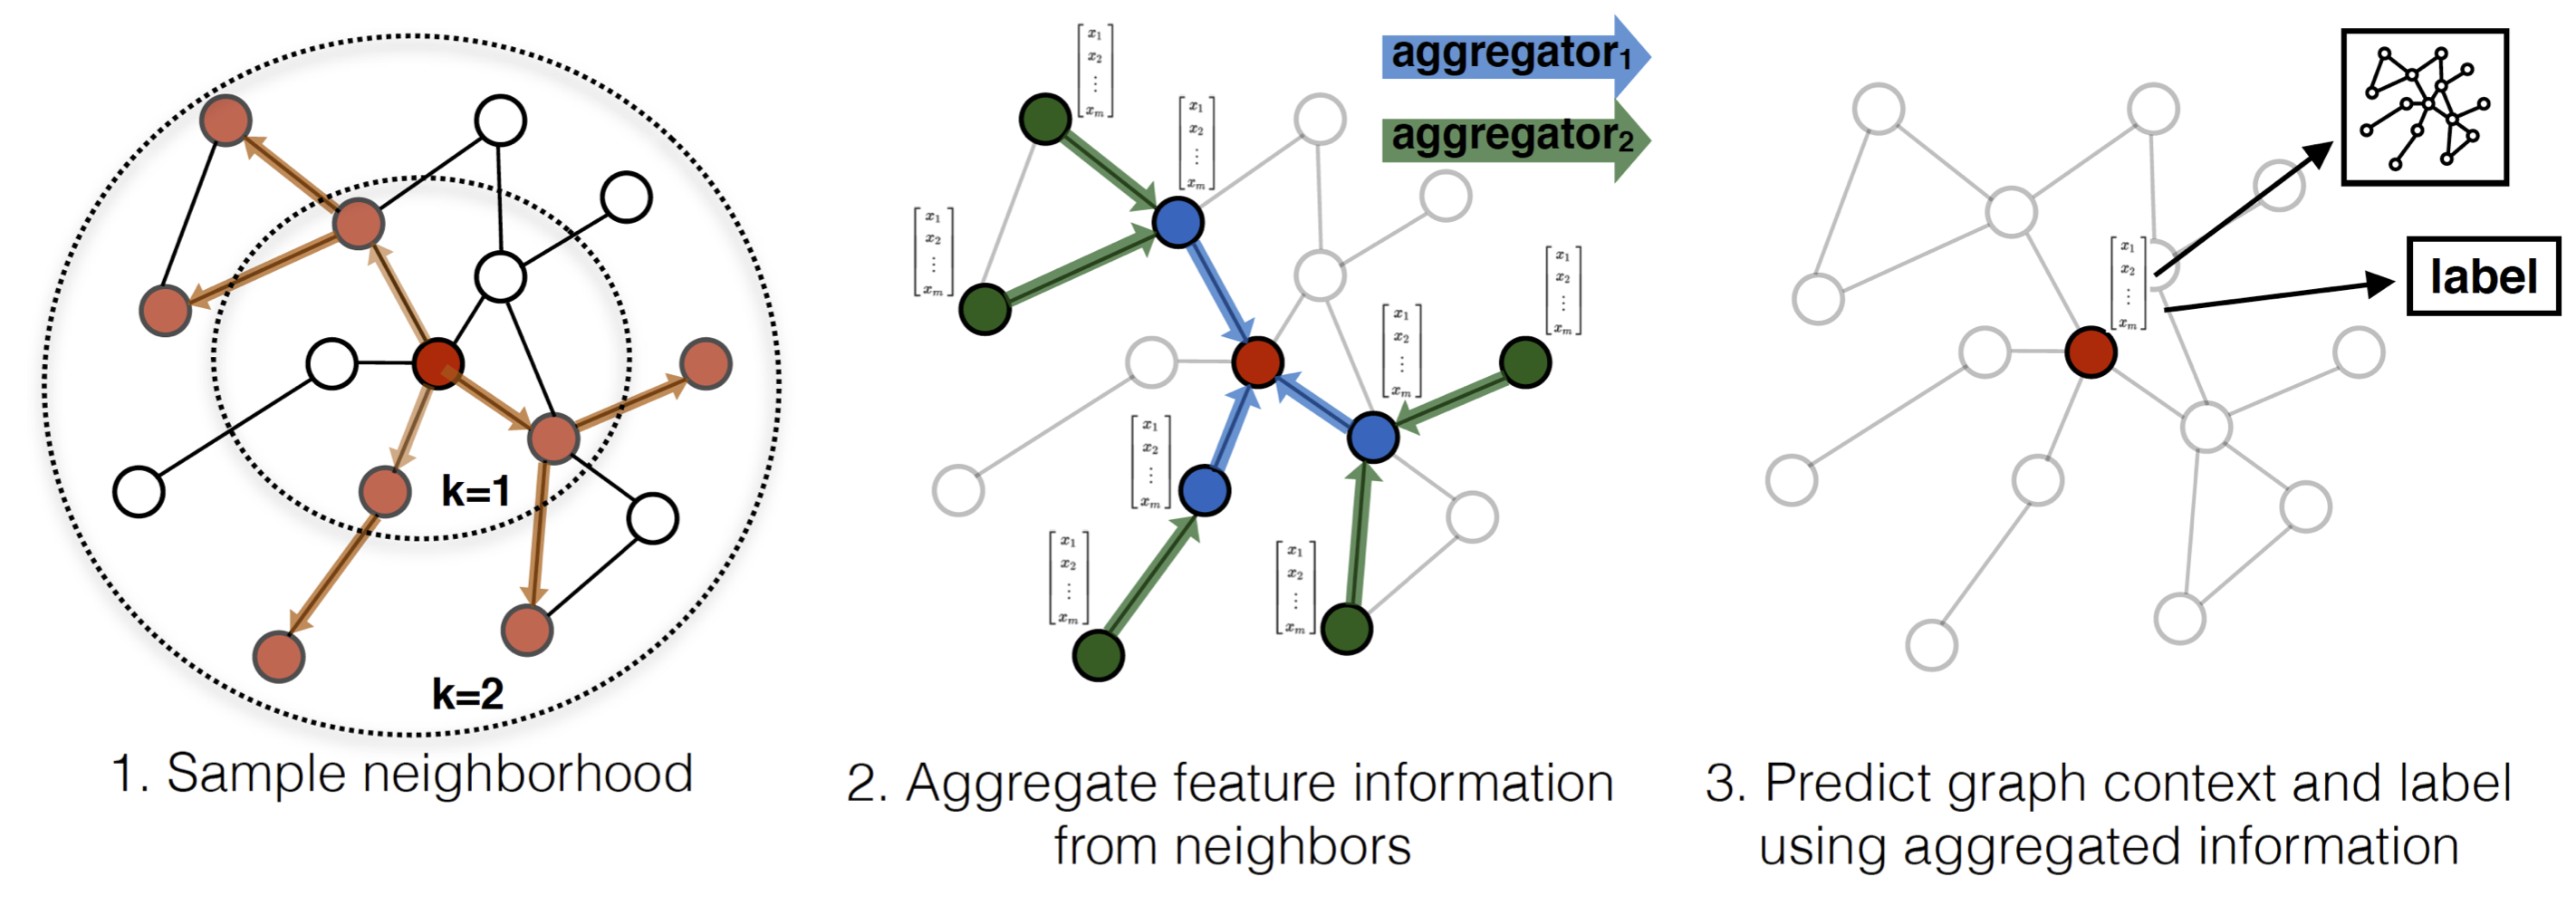
\includegraphics[width=0.8\textwidth]{sample_and_agg.png}
    \caption{Minh họa quy trình lấy mẫu và tổng hợp (Sample and Aggregate) của GraphSAGE}
    \label{fig:sample_and_agg}
\end{figure}

\subsection{Các hàm tổng hợp (Aggregators)}

GraphSAGE hỗ trợ nhiều loại hàm tổng hợp khác nhau, mỗi loại có những đặc điểm riêng:
\begin{itemize}
    \item \textbf{Mean Aggregator:} Tính trung bình cộng các vector đặc trưng của láng giềng. Đây là cách tiếp cận đơn giản và hiệu quả nhất, tương tự như phép tích chập trên đồ thị.
    \item \textbf{Pooling Aggregator:} Đưa các vector láng giềng qua một lớp kết nối đầy đủ (MLP) và thực hiện phép lấy cực đại (element-wise max pooling) để chọn lọc những đặc trưng nổi bật nhất.
    \item \textbf{LSTM Aggregator:} Sử dụng mạng LSTM để tổng hợp thông tin. Tuy nhiên, do LSTM không có tính bất biến với thứ tự (permutation invariant), các láng giềng cần được xáo trộn ngẫu nhiên trước khi đưa vào.
\end{itemize}

Trong đề tài này, hàm \textbf{Mean Aggregator} được ưu tiên sử dụng do tính đơn giản và khả năng tối ưu hóa tốt trên các thiết bị di động có tài nguyên hạn chế.

\section{Device-Cloud Collaborative Learning (DCCL)}

Học tập hợp tác thiết bị - đám mây (Device-Cloud Collaborative Learning - DCCL) là một kiến trúc hiện đại cho phép phân bổ linh hoạt các tác vụ tính toán và lưu trữ giữa máy chủ trung tâm (Cloud) và các thiết bị đầu cuối (Device). Trong bối cảnh hệ thống khuyến nghị, DCCL giải quyết mâu thuẫn giữa nhu cầu về tri thức toàn cục đồ sộ và yêu cầu bảo vệ quyền riêng tư, cá nhân hóa tức thời.

\subsection{Tổng quan kiến trúc}

Kiến trúc DCCL trong đề tài được thiết kế với sự phân định rõ ràng về vai trò của hai thành phần:

\begin{itemize}
    \item \textbf{Phía Đám mây (Cloud Server):}
    \begin{itemize}
        \item Lưu trữ và quản lý đồ thị tương tác toàn cục (Global Graph) bao gồm hàng triệu người dùng và sản phẩm.
        \item Thực hiện các tác vụ tính toán nặng: Huấn luyện mô hình GNN để học các vector nhúng (Global Embeddings).
        \item Cung cấp dịch vụ truy xuất ứng viên (Candidate Retrieval) dựa trên các thuật toán tìm kiếm láng giềng gần nhất (ANN) hoặc duyệt đồ thị.
    \end{itemize}
    \item \textbf{Phía Thiết bị (Device Client):}
    \begin{itemize}
        \item Lưu trữ đồ thị con cục bộ (Local Subgraph) chứa lịch sử tương tác gần nhất của người dùng.
        \item Lưu trữ mô hình ranking thu nhỏ (đã được tối ưu hóa bằng TFLite).
        \item Thực hiện tính toán xếp hạng (Ranking) ngay trên thiết bị để đưa ra kết quả khuyến nghị cuối cùng.
    \end{itemize}
\end{itemize}

\subsection{Ưu điểm của DCCL so với hệ thống truyền thống}

Kiến trúc phối hợp này mang lại nhiều lợi ích vượt trội:

\begin{table}[h!]
    \centering
    \caption{So sánh kiến trúc DCCL và kiến trúc Cloud-centric truyền thống}
    \renewcommand{\arraystretch}{1.5}
    \begin{tabularx}{\textwidth}{|l|X|X|}
        \hline
        \textbf{Tiêu chí} & \textbf{Cloud-centric truyền thống} & \textbf{DCCL (Đề xuất)} \\ \hline
        \textbf{Quyền riêng tư} & Dữ liệu hành vi thô phải đẩy lên Cloud. & Dữ liệu thô lưu tại thiết bị, chỉ truyền vector nhúng. \\ \hline
        \textbf{Băng thông} & Tốn nhiều băng thông để truyền log hành vi. & Tiết kiệm băng thông do chỉ truyền vector nhúng nhỏ gọn. \\ \hline
        \textbf{Độ trễ} & Phụ thuộc vào tốc độ mạng và tải của server. & Suy luận ranking tức thời tại thiết bị. \\ \hline
        \textbf{Cá nhân hóa} & Khó cập nhật sở thích tức thời. & Phản ánh hành vi thời gian thực cực kỳ nhạy bén. \\ \hline
    \end{tabularx}
    \label{tab:dccl_vs_traditional}
\end{table}

\subsection{Luồng inference trong hệ thống DCCL}

Quá trình đưa ra gợi ý cho người dùng trong hệ thống DCCL diễn ra qua các bước sau:

\begin{enumerate}
    \item \textbf{Khởi tạo yêu cầu:} Thiết bị gửi một mã định danh (User ID) lên Cloud khi người dùng bắt đầu phiên làm việc.
    \item \textbf{Truy xuất ứng viên (Cloud):} Đám mây dựa trên tri thức toàn cục để chọn ra một danh sách các sản phẩm tiềm năng (Candidates). Quá trình này thường kết hợp giữa duyệt đồ thị và tìm kiếm độ tương đồng vector.
    \item \textbf{Truyền tải tri thức:} Đám mây gửi danh sách ID ứng viên cùng với các vector nhúng (Item Embeddings) tương ứng về cho thiết bị.
    \item \textbf{Xếp hạng cục bộ (Device):} Thiết bị sử dụng mô hình TFLite để kết hợp Item Embeddings từ Cloud với đặc trưng từ Local Subgraph (lịch sử vừa xem) để tính toán điểm số ranking.
    \item \textbf{Hiển thị kết quả:} Kết quả có điểm số cao nhất được hiển thị tức thời cho người dùng.
\end{enumerate}

\section{Các độ đo và phương pháp đánh giá}

Để đánh giá hiệu quả của mô hình và hệ thống khuyến nghị được đề xuất, dự án tập trung vào hai khía cạnh chính: khả năng dự đoán liên kết của mô hình GNN và khả năng xếp hạng danh sách sản phẩm trên thiết bị.

\subsection{Area Under the ROC Curve (AUROC)}
AUROC đo lường khả năng của mô hình trong việc phân biệt giữa các cặp tương tác thực (positive edges) và các cặp tương tác giả (negative edges). Đây là độ đo cốt lõi được sử dụng trong quá trình huấn luyện và so sánh giữa kiến trúc GraphSAGE và GCN. Giá trị AUROC tiệm cận 1.0 thể hiện mô hình có khả năng dự đoán chính xác sự tồn tại của một liên kết giữa người dùng và sản phẩm.

\subsection{Average Precision (AP)}
AP đánh giá chất lượng của mô hình thông qua việc tính toán diện tích dưới đường cong Precision-Recall. Độ đo này đặc biệt hữu ích trong bài toán khuyến nghị khi chúng ta quan tâm đến việc các sản phẩm liên quan thực sự có được mô hình xếp hạng ở các vị trí cao hay không.
\begin{equation}
    \text{AP} = \sum_n (R_n - R_{n-1}) P_n
\end{equation}

\subsection{Cơ chế xếp hạng Top-K Recommendation}
Trong giai đoạn suy luận trên thiết bị (Inference), sau khi mô hình tính toán điểm số (logits) cho danh sách các sản phẩm ứng viên, hệ thống thực hiện xếp hạng và chỉ trả về $K$ sản phẩm có điểm số cao nhất.
\begin{equation}
    \mathcal{L}_{\text{rec}} = \text{argtopk}_{i \in \mathcal{I}} (\hat{y}_{u,i})
\end{equation}
Trong đó $K$ là số lượng gợi ý hiển thị cho người dùng (mặc định $K=5$ trong hiện thực thực tế của thiết bị). Việc sử dụng Top-K giúp tối ưu hóa không gian hiển thị và giảm tải tính toán cho thiết bị di động.

% -- CHƯƠNG 3: Các nghiên cứu liên quan
\chapter{CÁC NGHIÊN CỨU LIÊN QUAN}

\section{Giới thiệu các kỹ thuật giải quyết chủ đề}

Trong những năm gần đây, hệ thống khuyến nghị đã và đang chuyển dịch từ kiến trúc tập trung hoàn toàn trên đám mây (Cloud-centric) sang kiến trúc học hợp tác giữa thiết bị và đám mây (Device-Cloud Collaborative Learning - DCCL) nhằm giải quyết các hạn chế về quyền riêng tư, độ trễ và chi phí băng thông. Sự phát triển này thu hút sự quan tâm của nhiều nhóm nghiên cứu cũng như các kỹ sư hệ thống từ các công ty công nghệ hàng đầu, dẫn đến việc đề xuất hàng loạt các kỹ thuật và framework đa dạng. 

Dựa trên các nghiên cứu nổi bật được phân tích trong đề tài, các kỹ thuật giải quyết chủ đề khuyến nghị học hợp tác thiết bị - đám mây có thể được tổng hợp thành các hướng tiếp cận chính như sau:

\begin{itemize}
    \item \textbf{Phân tán tính toán và học hợp tác (Collaborative Learning):} Đây là kỹ thuật nền tảng cho kiến trúc DCCL, đề xuất việc tách biệt mô hình thành phần trên đám mây (lưu trữ và học đặc trưng toàn cục) và phần trên thiết bị (cá nhân hóa dựa trên đồ thị cục bộ). Phương pháp này giúp giảm tải việc truyền dữ liệu thô, thay vào đó hệ thống chỉ trao đổi các biểu diễn (embeddings) hoặc tham số trọng số, từ đó tối ưu băng thông và bảo vệ quyền riêng tư \cite{yao2021device}.
    
    \item \textbf{Học siêu tham số và tối ưu hóa thích ứng (Meta Learning / Meta Controller):} Để khắc phục vấn đề dữ liệu trên từng thiết bị đơn lẻ bị thưa thớt (sparsity) và biến động liên tục, các tác giả đề xuất sử dụng phương pháp Meta-Learning. Trong đó, đám mây không chỉ cung cấp mô hình chung mà còn cung cấp một mô hình điều khiển (Meta Controller) giúp thiết bị học cách thích ứng nhanh chóng với sự thay đổi trong sở thích của người dùng ngay cả khi chỉ có một lượng nhỏ dữ liệu tương tác mới nhất \cite{yao2022meta}.
    
    \item \textbf{Cơ chế hiệu chỉnh hợp tác (Collaborative Correction):} Các mô hình chạy trực tiếp trên thiết bị thường gặp phải hiện tượng chệch (bias) do chúng chỉ tiếp xúc với một vùng nhỏ của dữ liệu cục bộ thay vì cái nhìn toàn cảnh của đám mây. Kỹ thuật hiệu chỉnh hợp tác ra đời để giải quyết vấn đề này. Đám mây sẽ tính toán và gửi các tín hiệu hiệu chỉnh (correction signals) xuống thiết bị để tinh chỉnh quá trình dự đoán xếp hạng (ranking), đảm bảo tính chính xác toàn cục nhưng vẫn giữ được độ trễ thấp của on-device inference \cite{wang2025correction}.
    
    \item \textbf{Thiết kế hệ thống và nền tảng sản xuất (Production Systems):} Bên cạnh việc tối ưu thuật toán, một hướng kỹ thuật quan trọng khác là việc xây dựng hạ tầng phần mềm thực tế để có thể triển khai DCCL trên quy mô hàng tỷ thiết bị. Tiêu biểu là việc phát triển các hệ thống end-to-end (như hệ thống Walle), cung cấp một pipeline hoàn chỉnh từ bước xử lý dữ liệu, lên lịch huấn luyện, cho đến triển khai mô hình trên nhiều dòng thiết bị phần cứng khác nhau, đóng vai trò như một môi trường thực thi vững chắc cho các thuật toán DCCL \cite{cheng2022walle}.
\end{itemize}

Các kỹ thuật này không tồn tại độc lập mà thường bổ trợ lẫn nhau, tạo thành một hệ sinh thái hoàn chỉnh giúp hệ thống khuyến nghị đáp ứng được các yêu cầu khắt khe của môi trường thực tế. Trong các phần tiếp theo, chương này sẽ tổ chức và đánh giá chi tiết hơn về các đóng góp cũng như ưu, nhược điểm của từng nghiên cứu cụ thể.

\section{Các nghiên cứu liên quan theo thời gian}

Sự phát triển của kiến trúc hệ thống khuyến nghị học hợp tác thiết bị - đám mây (DCCL) có thể được quan sát rõ nét qua tiến trình thời gian từ khi hình thành ý tưởng cơ bản cho đến khi mở rộng thành các hệ thống thương mại phức tạp. Dưới đây là lộ trình phát triển qua các năm dựa trên các nghiên cứu tiêu biểu:

\subsection{Giai đoạn khởi nguồn (2021)}
Năm 2021 đánh dấu những bước đi đầu tiên trong việc hệ thống hóa kiến trúc DCCL cho hệ thống khuyến nghị. Nghiên cứu của \cite{yao2021device} đã đặt nền móng với giải pháp phân tách mô hình tính toán. Bằng cách giữ phần lớn mô hình (heavy model) trên đám mây để học biểu diễn toàn cục và đưa phần xếp hạng (ranking) xuống thiết bị di động, nghiên cứu này đã chứng minh tính khả thi của việc vừa giảm thiểu độ trễ, tiết kiệm băng thông, vừa bảo vệ quyền riêng tư do không cần tải dữ liệu thô của người dùng lên máy chủ.

\subsection{Giai đoạn mở rộng thuật toán và hiện thực hệ thống (2022)}
Đến năm 2022, trọng tâm nghiên cứu dịch chuyển từ việc thiết lập cấu trúc cơ bản sang giải quyết các bài toán hẹp, cụ thể hơn và đưa DCCL vào sản xuất thực tế:
\begin{itemize}
    \item \textbf{Cá nhân hóa và tối ưu hóa dữ liệu thưa:} Kế thừa những ưu điểm của kiến trúc DCCL, \cite{yao2022meta} nhận thấy thách thức của các mô hình trên thiết bị khi phải học với tập dữ liệu cục bộ nhỏ và biến động. Việc áp dụng Meta Learning để xây dựng một Meta Controller từ đám mây đã giúp thiết bị nhanh chóng hội tụ và thích nghi với sự dịch chuyển sở thích của người dùng.
    \item \textbf{Cơ sở hạ tầng quy mô lớn:} Đi song song với sự tiến bộ về mặt thuật toán là sự hoàn thiện về nền tảng hệ thống. Sự ra đời của hệ thống Walle \cite{cheng2022walle} là một cột mốc kỹ thuật quan trọng. Hệ thống này cung cấp một pipeline tự động hóa từ phân phối tác vụ, quản lý mô hình đến đồng bộ hóa trọng số giữa đám mây và hàng tỷ thiết bị biên với các cấu hình phần cứng khác nhau.
\end{itemize}

\subsection{Giai đoạn tinh chỉnh và giải quyết chệch toàn cục (2025)}
Khi DCCL được áp dụng rộng rãi, những hạn chế về độ chệch (bias) của mô hình chạy cục bộ ngày càng lộ rõ. Do các thiết bị chỉ nhìn thấy dữ liệu của người dùng hiện tại, kết quả ranking đôi khi thiếu sự đa dạng và mất đi tính chính xác so với mô hình toàn cục. Gần đây nhất, nghiên cứu về cơ chế hiệu chỉnh hợp tác \cite{wang2025correction} ra đời nhằm khắc phục nhược điểm này. Việc đám mây chủ động tính toán và gửi các tín hiệu hiệu chỉnh xuống thiết bị đánh dấu một bước tiến mới, tối ưu hóa sự cân bằng giữa khả năng cá nhân hóa tại thiết bị (on-device personalization) và góc nhìn toàn cảnh từ đám mây (global perspective).

\section{Đánh giá ưu nhược điểm của các nghiên cứu}

Việc phân tích chuyên sâu các điểm mạnh và điểm yếu của từng kỹ thuật giúp hệ thống hóa những ưu điểm kế thừa được, cũng như nhận diện các thách thức còn tồn đọng khi áp dụng kiến trúc DCCL.

\subsection{Device-Cloud Collaborative Learning for Recommendation \cite{yao2021device}}

Là một trong những nghiên cứu mang tính định hình kiến trúc học hợp tác thiết bị - đám mây cho bài toán khuyến nghị, giải pháp này mang lại những đột phá lớn nhưng cũng tồn tại những giới hạn kỹ thuật nhất định.

\textbf{Điểm mạnh:}
\begin{itemize}
    \item \textbf{Bảo mật và quyền riêng tư (Privacy-preserving):} Thay vì tải toàn bộ log hành vi của người dùng (click, view, v.v.) lên máy chủ tập trung như truyền thống, kiến trúc này giữ mọi dữ liệu thô ở lại thiết bị. Việc giao tiếp giữa thiết bị và đám mây chỉ thông qua các vector nhúng (embeddings) hoặc các tham số mô hình đã mã hóa, giúp hạn chế tối đa nguy cơ rò rỉ thông tin cá nhân.
    \item \textbf{Độ trễ suy luận thấp (Low Latency):} Bằng cách triển khai mô hình xếp hạng (ranking) trực tiếp lên thiết bị di động, quá trình tính toán điểm số và sắp xếp các ứng viên diễn ra cục bộ. Cơ chế này loại bỏ sự phụ thuộc vào đường truyền mạng trong pha xếp hạng, mang lại trải nghiệm tương tác với độ trễ gần như bằng không.
    \item \textbf{Khả năng cá nhân hóa thời gian thực:} Mô hình cục bộ có thể cập nhật và phản ứng ngay lập tức với các thao tác mới nhất của người dùng trong phiên làm việc hiện tại, thay vì phải đợi máy chủ đám mây tính toán và đồng bộ theo từng chu kỳ (batch processing).
\end{itemize}

\textbf{Điểm yếu:}
\begin{itemize}
    \item \textbf{Hiện tượng chệch dữ liệu cục bộ (Local Bias):} Do mô hình trên thiết bị chỉ được tinh chỉnh dựa trên một lượng nhỏ dữ liệu tương tác của một cá nhân, nó rất dễ gặp phải tình trạng quá khớp (overfitting) với sở thích ngắn hạn, dẫn đến việc thiếu đa dạng hóa và bỏ qua các xu hướng chung (global knowledge) đang phổ biến.
    \item \textbf{Rào cản về tài nguyên phần cứng:} Mặc dù phần xếp hạng đã được tinh gọn, việc phải tải, lưu trữ và tính toán trên các vector nhúng (đôi khi lên đến hàng trăm chiều) vẫn tạo ra áp lực lớn về bộ nhớ và thời lượng pin đối với các thiết bị di động có cấu hình thấp (low-end devices).
    \item \textbf{Phụ thuộc vào đám mây cho khâu sinh ứng viên (Candidate Retrieval):} Kiến trúc này chưa thể hoạt động độc lập hoàn toàn. Do không thể lưu trữ hàng triệu sản phẩm tại thiết bị, quá trình tìm kiếm ứng viên ban đầu vẫn bắt buộc phải gọi lên đám mây, đồng nghĩa với việc vẫn cần sự ổn định của kết nối mạng ở giai đoạn đầu của phễu khuyến nghị.
\end{itemize}

\subsection{Device-Cloud Collaborative Recommendation via Meta Learning \cite{yao2022meta}}

Nhận thấy hạn chế về mặt dữ liệu cục bộ của kiến trúc DCCL cơ bản, nghiên cứu này đề xuất tích hợp phương pháp Meta-Learning (học cách học) thông qua một Meta Controller trên đám mây, giúp mô hình trên thiết bị thích nghi nhanh chóng với dữ liệu mới.

\textbf{Điểm mạnh:}
\begin{itemize}
    \item \textbf{Giải quyết bài toán dữ liệu thưa (Data Sparsity):} Thiết bị di động thường chỉ lưu trữ một lịch sử tương tác rất ngắn. Bằng cách áp dụng Meta-Learning, mô hình đạt được khả năng học qua một vài mẫu (Few-shot learning), giúp nó nhanh chóng nắm bắt được sự dịch chuyển trong sở thích của người dùng mà không đòi hỏi lượng lớn dữ liệu tương tác.
    \item \textbf{Cân bằng giữa tri thức toàn cục và cục bộ:} Meta Controller đóng vai trò như một cầu nối, mang theo những tín hiệu tổng quát (global knowledge) từ đám mây xuống để điều khiển và khởi tạo trọng số cho mạng nơ-ron trên thiết bị. Điều này giúp giảm thiểu đáng kể hiện tượng chệch (local bias) đặc trưng của các hệ thống on-device.
    \item \textbf{Tối ưu hóa băng thông truyền tải:} Việc hệ thống trao đổi các tham số của Meta Controller và vector nhúng thay vì đồng bộ toàn bộ trọng số của một mô hình khổng lồ giúp duy trì sự tối ưu về băng thông mạng, phù hợp với môi trường di động.
\end{itemize}

\textbf{Điểm yếu:}
\begin{itemize}
    \item \textbf{Chi phí huấn luyện khổng lồ tại đám mây:} Phương pháp Meta-Learning thường yêu cầu quy trình tối ưu hóa hai vòng lặp lồng nhau (inner-loop và outer-loop) hoặc tính toán đạo hàm bậc hai. Điều này tiêu tốn cực kỳ nhiều tài nguyên tính toán và thời gian huấn luyện tại máy chủ đám mây.
    \item \textbf{Tính ổn định và nhạy cảm (Instability):} Các mô hình Meta-Learning vốn nổi tiếng là nhạy cảm với việc thiết lập siêu tham số. Trong môi trường thương mại điện tử thực tế với sự đa dạng hành vi cực lớn và dữ liệu chứa nhiều nhiễu (noise), việc đảm bảo mô hình luôn hội tụ ổn định cho hàng triệu thiết bị khác nhau là một rủi ro lớn.
\end{itemize}

\subsection{Walle: Hệ thống sản xuất quy mô lớn cho DCCL \cite{cheng2022walle}}

Khác với các nghiên cứu tập trung vào thuật toán, Walle đóng vai trò là một nền tảng cơ sở hạ tầng phần mềm (framework/system), được thiết kế nhằm đưa kiến trúc học hợp tác thiết bị - đám mây vào thực tiễn môi trường sản xuất với quy mô hàng tỷ thiết bị biên.

\textbf{Điểm mạnh:}
\begin{itemize}
    \item \textbf{Tính toàn vẹn (End-to-End \& General-Purpose):} Walle cung cấp một pipeline hoàn chỉnh bao phủ từ khâu thu thập dữ liệu, phân phối tác vụ (task distribution) đến triển khai và giám sát mô hình. Nó không bị giới hạn chỉ ở bài toán khuyến nghị mà còn hỗ trợ tính toán cho nhiều tác vụ học máy đa dạng khác.
    \item \textbf{Khả năng mở rộng quy mô (Large-Scale Scalability):} Hệ thống được kiến trúc để quản lý và đồng bộ mô hình trên hàng tỷ thiết bị đồng thời một cách đáng tin cậy. Đây là một đặc điểm thiết yếu để có thể triển khai thực tế trên các siêu ứng dụng thương mại điện tử.
    \item \textbf{Xử lý phân mảnh phần cứng (Hardware Heterogeneity):} Thiết bị di động của người dùng rất đa dạng về cấu hình. Walle có khả năng nhận diện sức mạnh tính toán, trạng thái pin và kết nối mạng của từng thiết bị, từ đó linh hoạt lên lịch (schedule) các tác vụ suy luận sao cho không làm treo máy hoặc sụt pin của người dùng.
\end{itemize}

\textbf{Điểm yếu:}
\begin{itemize}
    \item \textbf{Chi phí triển khai và vận hành cực kỳ lớn:} Việc xây dựng, duy trì và vận hành một hệ thống phân tán đồ sộ như Walle đòi hỏi nền tảng máy chủ đám mây khổng lồ và nguồn lực kỹ sư chuyên sâu, nằm ngoài tầm với của hầu hết các dự án và doanh nghiệp vừa và nhỏ.
    \item \textbf{Tính nội bộ và khó tiếp cận (Proprietary System):} Là một hệ thống sản xuất phục vụ hệ sinh thái doanh nghiệp khép kín, các thành phần cốt lõi của Walle không được mã nguồn mở hoàn toàn. Điều này gây khó khăn cho cộng đồng học thuật trong việc tái tạo (reproduce), kiểm chứng độc lập hoặc áp dụng vào các nghiên cứu mới.
\end{itemize}

\subsection{Device-Cloud Collaborative Correction for On-Device Recommendation \cite{wang2025correction}}

Nghiên cứu này ra đời nhằm trực tiếp giải quyết vấn đề độ chệch (local bias) của mô hình chạy trên thiết bị bằng cách thiết lập một cơ chế hiệu chỉnh (correction mechanism) chủ động từ đám mây.

\textbf{Điểm mạnh:}
\begin{itemize}
    \item \textbf{Nâng cao độ chính xác toàn cục (Global Accuracy):} Bằng cách tính toán và gửi các "tín hiệu hiệu chỉnh" từ mô hình khổng lồ trên đám mây xuống thiết bị, hệ thống giúp tinh chỉnh lại kết quả xếp hạng cục bộ. Điều này đảm bảo danh sách gợi ý không bị giới hạn trong sở thích ngắn hạn mà còn phản ánh được các xu hướng chung, cải thiện tính đa dạng của kết quả.
    \item \textbf{Hiệu quả về chi phí truyền tải:} Tín hiệu hiệu chỉnh thường chỉ là các tham số vô hướng (scalars) hoặc các vector có số chiều thấp. Truyền tải các tín hiệu này tối ưu băng thông hơn rất nhiều so với việc tải xuống toàn bộ cấu trúc mô hình mới.
    \item \textbf{Tính mô-đun hóa (Modularity):} Cơ chế hiệu chỉnh này hoạt động như một module cắm thêm (plug-and-play), có thể tích hợp linh hoạt lên trên các kiến trúc DCCL hiện tại mà không làm phá vỡ kiến trúc cốt lõi đã có.
\end{itemize}

\textbf{Điểm yếu:}
\begin{itemize}
    \item \textbf{Nguy cơ gia tăng độ trễ (Latency Risk):} Nếu cơ chế hiệu chỉnh đòi hỏi thiết bị phải chờ tín hiệu từ đám mây trước khi đưa ra kết quả cuối cùng cho người dùng, điều này sẽ làm mất đi ưu điểm lớn nhất của on-device inference là tốc độ phản hồi tức thời (real-time), đặc biệt trong điều kiện mạng yếu.
    \item \textbf{Thách thức trong việc cân bằng trọng số (Weight Balancing):} Việc quyết định mức độ tác động của tín hiệu hiệu chỉnh lên kết quả cục bộ là một bài toán khó. Nếu hiệu chỉnh quá mạnh, hệ thống sẽ đánh mất tính cá nhân hóa; ngược lại, nếu quá yếu, quá trình hiệu chỉnh sẽ trở nên vô nghĩa và lãng phí băng thông.
\end{itemize}

% -- CHƯƠNG 4: Thực nghiệm
\chapter{THỰC NGHIỆM}

\section{Giới thiệu Dataset}

\subsection{Ali-CCP (Alibaba Click-Conversion Prediction)}
% TODO: Mô tả chi tiết dataset.
% Gợi ý:
%   - Nguồn: Alibaba Tianchi Platform.
%   - Quy mô: Số mẫu, số người dùng, số sản phẩm, thời gian thu thập.
%   - Cấu trúc: user_id, item_id, timestamp, label (click/purchase), device features.
%   - Tại sao chọn: Dataset thực tế từ chính Alibaba - đơn vị tiên phong DCCL.
%   - Thống kê cơ bản (bảng hoặc biểu đồ): Phân phối rating, sparsity, ...

\subsection{Tiền xử lý dữ liệu}
% TODO: Mô tả các bước tiền xử lý.
% Gợi ý:
%   - Lọc người dùng/sản phẩm có ít tương tác (K-core filtering).
%   - Chia tập train/validation/test (theo thời gian - temporal split).
%   - Xây dựng đồ thị tương tác: Node = User + Item, Edge = Interaction.
%   - So sánh dung lượng: Dữ liệu thô vs. Embeddings (minh họa lợi ích DCCL).

\section{Sơ đồ thiết kế thực nghiệm}

\subsection{Kiến trúc hệ thống tổng thể}
% TODO: Chèn hình kiến trúc hệ thống DCCL.
% Gợi ý nội dung hình:
%   - Cloud Server: GNN Training (GraphSAGE) → Item Embedding Store → Candidate API.
%   - Device Client: Local Subgraph → TFLite Ranker → Recommendations.
%   - Kênh giao tiếp: REST API (JSON).

% \begin{figure}[h!]
%     \centering
%     \includegraphics[width=0.85\textwidth]{figures/system_architecture.png}
%     \caption{Kiến trúc tổng thể hệ thống Device-Cloud Collaborative Learning}
%     \label{fig:architecture}
% \end{figure}

\subsection{Lưu đồ giải thuật}
% TODO: Vẽ lưu đồ minh họa quy trình inference end-to-end.
% Gợi ý (dùng tikz hoặc chèn hình):
%   Bước 1: Device gửi {user_id, k} lên Cloud.
%   Bước 2: Cloud thực hiện 3-stage retrieval (Graph → Vector → Popularity).
%   Bước 3: Cloud trả về {candidate_ids, embeddings}.
%   Bước 4: Device ranking bằng TFLite model.
%   Bước 5: Trả kết quả Top-K cho người dùng.

\section{Các phương pháp đánh giá}

% TODO: Mô tả 3-4 metrics sẽ sử dụng.

\subsection{Precision@K}
% Công thức: P@K = (số items liên quan trong top-K) / K

\subsection{Recall@K}
% Công thức: R@K = (số items liên quan trong top-K) / (tổng số items liên quan)

\subsection{NDCG@K (Normalized Discounted Cumulative Gain)}
% Công thức: NDCG@K = DCG@K / IDCG@K
% Trong đó: DCG@K = \sum_{i=1}^{K} \frac{rel_i}{\log_2(i+1)}

\subsection{Hit Rate@K}
% Công thức: HR@K = 1 nếu item liên quan xuất hiện trong top-K, ngược lại 0.

\section{Mô tả thực nghiệm}

\subsection{Thiết lập thực nghiệm}
% TODO: Mô tả cấu hình thực nghiệm.
% Gợi ý:
%   - Phần cứng: CPU/GPU dùng để huấn luyện Cloud model, thiết bị mô phỏng Device.
%   - Thư viện: PyTorch Geometric (PyG), TensorFlow Lite, FastAPI.
%   - Siêu tham số: Số lớp GNN, kích thước embedding, learning rate, batch size, epochs.
%   - Baseline so sánh: BPR-MF, LightGCN, PureSVD.

\subsection{Kết quả thực nghiệm}
% TODO: Trình bày kết quả dưới dạng bảng so sánh.

\begin{table}[h!]
    \centering
    \caption{Kết quả so sánh hiệu năng giữa các phương pháp trên tập test}
    \renewcommand{\arraystretch}{1.4}
    \begin{tabularx}{\textwidth}{|l|X|X|X|X|}
        \hline
        \textbf{Phương pháp} & \textbf{Precision@10} & \textbf{Recall@10} & \textbf{NDCG@10} & \textbf{HR@10} \\ \hline
        BPR-MF       & --    & --    & --    & -- \\ \hline
        LightGCN     & --    & --    & --    & -- \\ \hline
        DCCL (Nhóm)  & --    & --    & --    & -- \\ \hline
    \end{tabularx}
    \label{tab:results}
\end{table}

\subsection{Phân tích kết quả}
% TODO: Nhận xét và phân tích kết quả từ bảng so sánh.
% Gợi ý:
%   - So sánh hệ thống DCCL của nhóm với các baseline.
%   - Phân tích ảnh hưởng của k (số ứng viên) đến chất lượng khuyến nghị.
%   - Vẽ biểu đồ: Bar chart hoặc line chart thể hiện Precision/NDCG theo K.

% \begin{figure}[h!]
%     \centering
%     \includegraphics[width=0.75\textwidth]{figures/ndcg_comparison.png}
%     \caption{So sánh NDCG@K của các phương pháp}
%     \label{fig:ndcg}
% \end{figure}

\subsection{Phân tích chi phí truyền thông}
% TODO: So sánh băng thông cần thiết giữa truyền dữ liệu thô và truyền embeddings.
% Gợi ý (vẽ biểu đồ cột):
%   - Truyền dữ liệu thô: X MB/request
%   - Truyền embeddings: Y KB/request
%   => Tiết kiệm Z lần băng thông.

% -- CHƯƠNG 5: Kết luận
\chapter{KẾT LUẬN}

\section{Tóm tắt đề tài}
% TODO: Nhắc lại bài toán và mục tiêu đề ra từ Chương 1.
% Gợi ý:
%   - Đề tài nghiên cứu và hiện thực hệ thống khuyến nghị theo mô hình
%     Device-Cloud Collaborative Learning (DCCL) dựa trên Graph Neural Networks.
%   - Bài toán: Xây dựng pipeline hoàn chỉnh bảo vệ quyền riêng tư người dùng,
%     giảm băng thông, đồng thời đảm bảo chất lượng khuyến nghị cá nhân hóa cao.

\section{Tổng hợp các công việc đã thực hiện}
% TODO: Liệt kê tóm tắt những gì nhóm đã làm.
% Gợi ý (dùng itemize):
\begin{itemize}
    \item Khảo sát và hệ thống hóa lý thuyết về Graph Neural Networks (GraphSAGE)
    và cơ chế Device-Cloud Collaborative Learning.

    \item Nghiên cứu và phân tích 5 công trình tiêu biểu liên quan đến DCCL
    và GNN-based Recommendation, từ đó xác định hướng tiếp cận cho đề tài.

    \item Tiền xử lý và xây dựng đồ thị tương tác từ dataset Ali-CCP.

    \item Xây dựng Cloud Server:
    \begin{itemize}
        \item Huấn luyện mô hình 2-layer GraphSAGE để sinh Item Embeddings.
        \item Hiện thực 3-stage Candidate Retrieval API (Graph-based, Vector-based, Popularity).
    \end{itemize}

    \item Xây dựng Device Client:
    \begin{itemize}
        \item Chuyển đổi mô hình sang TFLite để thực hiện on-device inference.
        \item Hiện thực pipeline: nhận candidates từ Cloud → ranking cục bộ → trả kết quả.
    \end{itemize}

    \item Đánh giá hệ thống trên các metrics: Precision@K, Recall@K, NDCG@K, HR@K.
    \item So sánh với các phương pháp baseline và phân tích chi phí truyền thông.
\end{itemize}

\section{Ưu điểm và hạn chế}

\subsection{Ưu điểm}
% TODO: Nêu ưu điểm của hệ thống đã xây dựng.
\begin{itemize}
    \item \textbf{Bảo vệ quyền riêng tư:} Dữ liệu thô của người dùng không được
    truyền lên Cloud, chỉ truyền vector nhúng (embeddings).

    \item \textbf{Tiết kiệm băng thông:} [TODO: Điền con số cụ thể sau khi thực nghiệm]
    lần tiết kiệm so với truyền dữ liệu thô.

    \item \textbf{Độ trễ thấp:} Ranking được thực hiện cục bộ trên thiết bị,
    không phụ thuộc vào kết nối mạng tại thời điểm suy luận.

    \item \textbf{Pipeline hoàn chỉnh:} Đề tài hiện thực được end-to-end pipeline
    từ huấn luyện Cloud GNN đến on-device inference, có thể mở rộng.

    \item \textbf{Candidate Retrieval đa tầng:} Cơ chế 3-stage giúp đảm bảo tính
    đa dạng và liên quan của danh sách ứng viên.
\end{itemize}

\subsection{Hạn chế}
% TODO: Thành thật nêu các hạn chế còn tồn tại.
\begin{itemize}
    \item \textbf{Môi trường thực nghiệm giả lập:} Device được mô phỏng bằng máy tính,
    chưa triển khai thực sự trên phần cứng di động vật lý.

    \item \textbf{Chưa xử lý Cold-Start:} Hệ thống chưa có cơ chế xử lý hiệu quả
    cho người dùng mới hoặc sản phẩm mới.

    \item \textbf{Đồng bộ mô hình:} Cơ chế cập nhật mô hình từ Cloud xuống Device
    chưa được hiện thực tự động.

    \item \textbf{Quy mô dataset:} Thực nghiệm trên tập con của Ali-CCP do giới hạn
    tài nguyên tính toán, chưa phản ánh đầy đủ quy mô thực tế.
\end{itemize}

\section{Hướng phát triển trong tương lai}
% TODO: Đề xuất các hướng mở rộng.
\begin{itemize}
    \item \textbf{Federated Learning:} Tích hợp Federated Learning để Device có thể
    đóng góp vào quá trình huấn luyện mô hình toàn cục mà không cần chia sẻ dữ liệu thô.

    \item \textbf{On-device Model Update:} Hiện thực cơ chế cập nhật mô hình tự động
    khi có phiên bản mới từ Cloud.

    \item \textbf{Dynamic Graph:} Mở rộng mô hình GNN để xử lý đồ thị động
    (thêm/bớt cạnh theo thời gian thực).

    \item \textbf{Triển khai thực tế:} Đưa hệ thống lên phần cứng di động thực sự
    (Android với TFLite) để đo lường hiệu năng thực tế.

    \item \textbf{Multi-modal Features:} Tích hợp thêm đặc trưng hình ảnh/văn bản
    của sản phẩm vào quá trình học embedding.
\end{itemize}


\newpage
\addcontentsline{toc}{chapter}{Tài liệu tham khảo}
\renewcommand{\bibname}{Tài liệu tham khảo}
\nocite{*}
\bibliographystyle{plain}
\bibliography{references}

\end{document}
